% Created by tikzDevice version 0.12.6 on 2025-04-07 13:11:38
% !TEX encoding = UTF-8 Unicode
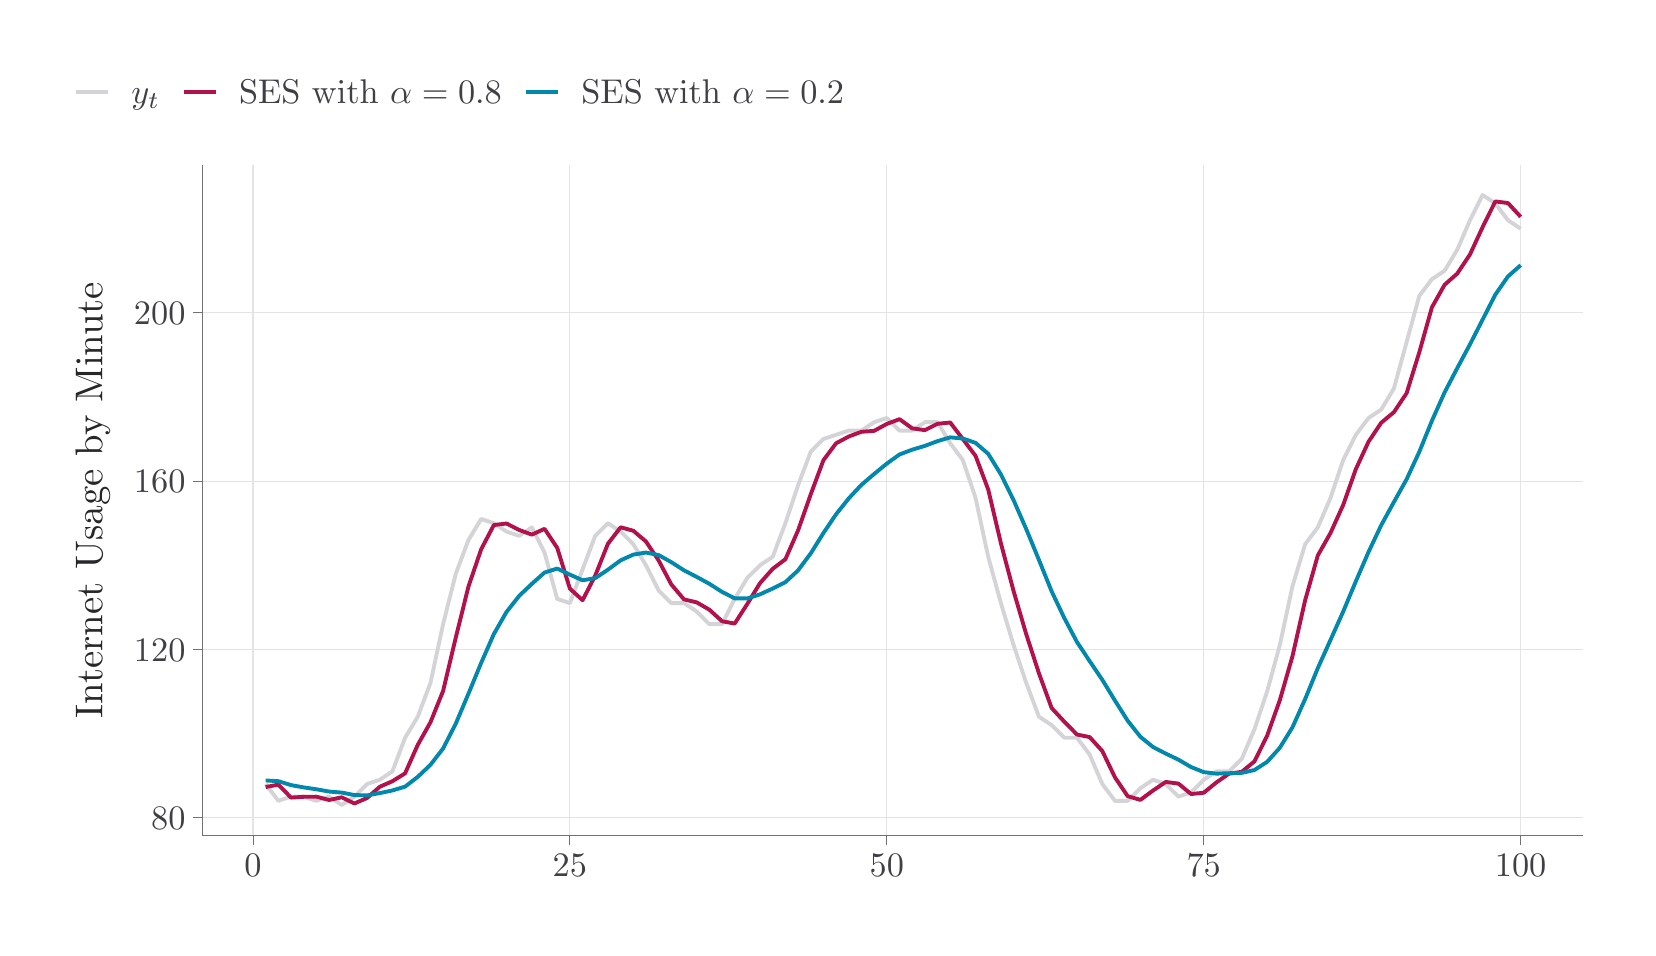
\begin{tikzpicture}[x=1pt,y=1pt]
\definecolor{fillColor}{RGB}{255,255,255}
\path[use as bounding box,fill=fillColor] (0,0) rectangle (578.16,325.21);
\begin{scope}
\path[clip] (  0.00,  0.00) rectangle (578.16,325.21);
\definecolor{drawColor}{RGB}{255,255,255}

\path[draw=drawColor,line width= 0.7pt,line join=round,line cap=round,fill=fillColor] (  0.00,  0.00) rectangle (578.16,325.21);
\end{scope}
\begin{scope}
\path[clip] ( 63.32, 33.29) rectangle (562.16,275.76);
\definecolor{drawColor}{RGB}{255,255,255}
\definecolor{fillColor}{RGB}{255,255,255}

\path[draw=drawColor,line width= 0.7pt,line join=round,line cap=round,fill=fillColor] ( 63.32, 33.29) rectangle (562.16,275.76);
\definecolor{drawColor}{RGB}{228,228,231}

\path[draw=drawColor,line width= 0.4pt,line join=round] ( 63.32, 39.75) --
	(562.16, 39.75);

\path[draw=drawColor,line width= 0.4pt,line join=round] ( 63.32,100.56) --
	(562.16,100.56);

\path[draw=drawColor,line width= 0.4pt,line join=round] ( 63.32,161.36) --
	(562.16,161.36);

\path[draw=drawColor,line width= 0.4pt,line join=round] ( 63.32,222.17) --
	(562.16,222.17);

\path[draw=drawColor,line width= 0.4pt,line join=round] ( 81.41, 33.29) --
	( 81.41,275.76);

\path[draw=drawColor,line width= 0.4pt,line join=round] (195.93, 33.29) --
	(195.93,275.76);

\path[draw=drawColor,line width= 0.4pt,line join=round] (310.45, 33.29) --
	(310.45,275.76);

\path[draw=drawColor,line width= 0.4pt,line join=round] (424.97, 33.29) --
	(424.97,275.76);

\path[draw=drawColor,line width= 0.4pt,line join=round] (539.49, 33.29) --
	(539.49,275.76);
\definecolor{drawColor}{RGB}{212,212,216}

\path[draw=drawColor,line width= 1.4pt,line join=round] ( 85.99, 51.91) --
	( 90.57, 45.83) --
	( 95.16, 47.35) --
	( 99.74, 47.35) --
	(104.32, 45.83) --
	(108.90, 47.35) --
	(113.48, 44.31) --
	(118.06, 47.35) --
	(122.64, 51.91) --
	(127.22, 53.43) --
	(131.80, 56.47) --
	(136.38, 68.63) --
	(140.96, 76.23) --
	(145.54, 88.39) --
	(150.12,109.68) --
	(154.70,127.92) --
	(159.29,140.08) --
	(163.87,147.68) --
	(168.45,146.16) --
	(173.03,143.12) --
	(177.61,141.60) --
	(182.19,144.64) --
	(186.77,135.52) --
	(191.35,118.80) --
	(195.93,117.28) --
	(200.51,129.44) --
	(205.09,141.60) --
	(209.67,146.16) --
	(214.25,143.12) --
	(218.83,138.56) --
	(223.42,130.96) --
	(228.00,121.84) --
	(232.58,117.28) --
	(237.16,117.28) --
	(241.74,114.24) --
	(246.32,109.68) --
	(250.90,109.68) --
	(255.48,118.80) --
	(260.06,126.40) --
	(264.64,130.96) --
	(269.22,134.00) --
	(273.80,146.16) --
	(278.38,159.84) --
	(282.96,172.01) --
	(287.55,176.57) --
	(292.13,178.09) --
	(296.71,179.61) --
	(301.29,179.61) --
	(305.87,182.65) --
	(310.45,184.17) --
	(315.03,179.61) --
	(319.61,179.61) --
	(324.19,182.65) --
	(328.77,182.65) --
	(333.35,175.05) --
	(337.93,168.97) --
	(342.51,155.28) --
	(347.09,134.00) --
	(351.68,117.28) --
	(356.26,102.08) --
	(360.84, 88.39) --
	(365.42, 76.23) --
	(370.00, 73.19) --
	(374.58, 68.63) --
	(379.16, 68.63) --
	(383.74, 62.55) --
	(388.32, 51.91) --
	(392.90, 45.83) --
	(397.48, 45.83) --
	(402.06, 50.39) --
	(406.64, 53.43) --
	(411.23, 51.91) --
	(415.81, 47.35) --
	(420.39, 48.87) --
	(424.97, 53.43) --
	(429.55, 56.47) --
	(434.13, 56.47) --
	(438.71, 61.03) --
	(443.29, 71.67) --
	(447.87, 85.35) --
	(452.45,102.08) --
	(457.03,123.36) --
	(461.61,138.56) --
	(466.19,144.64) --
	(470.77,155.28) --
	(475.36,168.97) --
	(479.94,178.09) --
	(484.52,184.17) --
	(489.10,187.21) --
	(493.68,194.81) --
	(498.26,211.53) --
	(502.84,228.25) --
	(507.42,234.34) --
	(512.00,237.38) --
	(516.58,244.98) --
	(521.16,255.62) --
	(525.74,264.74) --
	(530.32,261.70) --
	(534.90,255.62) --
	(539.49,252.58);
\definecolor{drawColor}{RGB}{179,17,75}

\path[draw=drawColor,line width= 1.4pt,line join=round] ( 85.99, 50.80) --
	( 90.57, 51.69) --
	( 95.16, 47.00) --
	( 99.74, 47.28) --
	(104.32, 47.33) --
	(108.90, 46.13) --
	(113.48, 47.10) --
	(118.06, 44.87) --
	(122.64, 46.85) --
	(127.22, 50.90) --
	(131.80, 52.92) --
	(136.38, 55.76) --
	(140.96, 66.06) --
	(145.54, 74.20) --
	(150.12, 85.55) --
	(154.70,104.85) --
	(159.29,123.31) --
	(163.87,136.73) --
	(168.45,145.49) --
	(173.03,146.03) --
	(177.61,143.70) --
	(182.19,142.02) --
	(186.77,144.12) --
	(191.35,137.24) --
	(195.93,122.49) --
	(200.51,118.32) --
	(205.09,127.22) --
	(209.67,138.72) --
	(214.25,144.67) --
	(218.83,143.43) --
	(223.42,139.54) --
	(228.00,132.68) --
	(232.58,124.01) --
	(237.16,118.62) --
	(241.74,117.55) --
	(246.32,114.90) --
	(250.90,110.72) --
	(255.48,109.89) --
	(260.06,117.02) --
	(264.64,124.52) --
	(269.22,129.67) --
	(273.80,133.13) --
	(278.38,143.56) --
	(282.96,156.59) --
	(287.55,168.92) --
	(292.13,175.04) --
	(296.71,177.48) --
	(301.29,179.18) --
	(305.87,179.52) --
	(310.45,182.02) --
	(315.03,183.74) --
	(319.61,180.43) --
	(324.19,179.77) --
	(328.77,182.07) --
	(333.35,182.53) --
	(337.93,176.54) --
	(342.51,170.48) --
	(347.09,158.32) --
	(351.68,138.87) --
	(356.26,121.60) --
	(360.84,105.98) --
	(365.42, 91.91) --
	(370.00, 79.37) --
	(374.58, 74.43) --
	(379.16, 69.79) --
	(383.74, 68.86) --
	(388.32, 63.81) --
	(392.90, 54.29) --
	(397.48, 47.52) --
	(402.06, 46.17) --
	(406.64, 49.54) --
	(411.23, 52.65) --
	(415.81, 52.06) --
	(420.39, 48.29) --
	(424.97, 48.75) --
	(429.55, 52.49) --
	(434.13, 55.67) --
	(438.71, 56.31) --
	(443.29, 60.09) --
	(447.87, 69.35) --
	(452.45, 82.15) --
	(457.03, 98.09) --
	(461.61,118.31) --
	(466.19,134.51) --
	(470.77,142.62) --
	(475.36,152.75) --
	(479.94,165.72) --
	(484.52,175.61) --
	(489.10,182.46) --
	(493.68,186.26) --
	(498.26,193.10) --
	(502.84,207.85) --
	(507.42,224.17) --
	(512.00,232.30) --
	(516.58,236.36) --
	(521.16,243.25) --
	(525.74,253.15) --
	(530.32,262.42) --
	(534.90,261.84) --
	(539.49,256.86);
\definecolor{drawColor}{RGB}{1,136,172}

\path[draw=drawColor,line width= 1.4pt,line join=round] ( 85.99, 53.19) --
	( 90.57, 52.93) --
	( 95.16, 51.51) --
	( 99.74, 50.68) --
	(104.32, 50.01) --
	(108.90, 49.18) --
	(113.48, 48.81) --
	(118.06, 47.91) --
	(122.64, 47.80) --
	(127.22, 48.62) --
	(131.80, 49.58) --
	(136.38, 50.96) --
	(140.96, 54.49) --
	(145.54, 58.84) --
	(150.12, 64.75) --
	(154.70, 73.74) --
	(159.29, 84.57) --
	(163.87, 95.68) --
	(168.45,106.08) --
	(173.03,114.09) --
	(177.61,119.90) --
	(182.19,124.24) --
	(186.77,128.32) --
	(191.35,129.76) --
	(195.93,127.57) --
	(200.51,125.51) --
	(205.09,126.30) --
	(209.67,129.36) --
	(214.25,132.72) --
	(218.83,134.80) --
	(223.42,135.55) --
	(228.00,134.63) --
	(232.58,132.07) --
	(237.16,129.12) --
	(241.74,126.75) --
	(246.32,124.25) --
	(250.90,121.33) --
	(255.48,119.00) --
	(260.06,118.96) --
	(264.64,120.45) --
	(269.22,122.55) --
	(273.80,124.84) --
	(278.38,129.10) --
	(282.96,135.25) --
	(287.55,142.60) --
	(292.13,149.40) --
	(296.71,155.13) --
	(301.29,160.03) --
	(305.87,163.94) --
	(310.45,167.69) --
	(315.03,170.98) --
	(319.61,172.71) --
	(324.19,174.09) --
	(328.77,175.80) --
	(333.35,177.17) --
	(337.93,176.74) --
	(342.51,175.19) --
	(347.09,171.21) --
	(351.68,163.77) --
	(356.26,154.47) --
	(360.84,143.99) --
	(365.42,132.87) --
	(370.00,121.54) --
	(374.58,111.87) --
	(379.16,103.22) --
	(383.74, 96.31) --
	(388.32, 89.55) --
	(392.90, 82.03) --
	(397.48, 74.79) --
	(402.06, 68.99) --
	(406.64, 65.27) --
	(411.23, 62.90) --
	(415.81, 60.71) --
	(420.39, 58.03) --
	(424.97, 56.20) --
	(429.55, 55.65) --
	(434.13, 55.81) --
	(438.71, 55.94) --
	(443.29, 56.96) --
	(447.87, 59.90) --
	(452.45, 64.99) --
	(457.03, 72.41) --
	(461.61, 82.60) --
	(466.19, 93.79) --
	(470.77,103.96) --
	(475.36,114.23) --
	(479.94,125.17) --
	(484.52,135.76) --
	(489.10,145.44) --
	(493.68,153.79) --
	(498.26,162.00) --
	(502.84,171.90) --
	(507.42,183.17) --
	(512.00,193.41) --
	(516.58,202.20) --
	(521.16,210.76) --
	(525.74,219.73) --
	(530.32,228.73) --
	(534.90,235.32) --
	(539.49,239.38);
\end{scope}
\begin{scope}
\path[clip] (  0.00,  0.00) rectangle (578.16,325.21);
\definecolor{drawColor}{RGB}{113,113,122}

\path[draw=drawColor,line width= 0.3pt,line join=round] ( 63.32, 33.29) --
	( 63.32,275.76);
\end{scope}
\begin{scope}
\path[clip] (  0.00,  0.00) rectangle (578.16,325.21);
\definecolor{drawColor}{RGB}{63,63,70}

\node[text=drawColor,anchor=base east,inner sep=0pt, outer sep=0pt, scale=  1.24] at ( 57.02, 35.46) {80};

\node[text=drawColor,anchor=base east,inner sep=0pt, outer sep=0pt, scale=  1.24] at ( 57.02, 96.27) {120};

\node[text=drawColor,anchor=base east,inner sep=0pt, outer sep=0pt, scale=  1.24] at ( 57.02,157.08) {160};

\node[text=drawColor,anchor=base east,inner sep=0pt, outer sep=0pt, scale=  1.24] at ( 57.02,217.89) {200};
\end{scope}
\begin{scope}
\path[clip] (  0.00,  0.00) rectangle (578.16,325.21);
\definecolor{drawColor}{RGB}{113,113,122}

\path[draw=drawColor,line width= 0.3pt,line join=round] ( 59.82, 39.75) --
	( 63.32, 39.75);

\path[draw=drawColor,line width= 0.3pt,line join=round] ( 59.82,100.56) --
	( 63.32,100.56);

\path[draw=drawColor,line width= 0.3pt,line join=round] ( 59.82,161.36) --
	( 63.32,161.36);

\path[draw=drawColor,line width= 0.3pt,line join=round] ( 59.82,222.17) --
	( 63.32,222.17);
\end{scope}
\begin{scope}
\path[clip] (  0.00,  0.00) rectangle (578.16,325.21);
\definecolor{drawColor}{RGB}{113,113,122}

\path[draw=drawColor,line width= 0.3pt,line join=round] ( 63.32, 33.29) --
	(562.16, 33.29);
\end{scope}
\begin{scope}
\path[clip] (  0.00,  0.00) rectangle (578.16,325.21);
\definecolor{drawColor}{RGB}{113,113,122}

\path[draw=drawColor,line width= 0.3pt,line join=round] ( 81.41, 29.79) --
	( 81.41, 33.29);

\path[draw=drawColor,line width= 0.3pt,line join=round] (195.93, 29.79) --
	(195.93, 33.29);

\path[draw=drawColor,line width= 0.3pt,line join=round] (310.45, 29.79) --
	(310.45, 33.29);

\path[draw=drawColor,line width= 0.3pt,line join=round] (424.97, 29.79) --
	(424.97, 33.29);

\path[draw=drawColor,line width= 0.3pt,line join=round] (539.49, 29.79) --
	(539.49, 33.29);
\end{scope}
\begin{scope}
\path[clip] (  0.00,  0.00) rectangle (578.16,325.21);
\definecolor{drawColor}{RGB}{63,63,70}

\node[text=drawColor,anchor=base,inner sep=0pt, outer sep=0pt, scale=  1.24] at ( 81.41, 18.42) {0};

\node[text=drawColor,anchor=base,inner sep=0pt, outer sep=0pt, scale=  1.24] at (195.93, 18.42) {25};

\node[text=drawColor,anchor=base,inner sep=0pt, outer sep=0pt, scale=  1.24] at (310.45, 18.42) {50};

\node[text=drawColor,anchor=base,inner sep=0pt, outer sep=0pt, scale=  1.24] at (424.97, 18.42) {75};

\node[text=drawColor,anchor=base,inner sep=0pt, outer sep=0pt, scale=  1.24] at (539.49, 18.42) {100};
\end{scope}
\begin{scope}
\path[clip] (  0.00,  0.00) rectangle (578.16,325.21);
\definecolor{drawColor}{RGB}{39,39,42}

\node[text=drawColor,rotate= 90.00,anchor=base,inner sep=0pt, outer sep=0pt, scale=  1.40] at ( 27.00,154.52) {Internet Usage by Minute};
\end{scope}
\begin{scope}
\path[clip] (  0.00,  0.00) rectangle (578.16,325.21);
\definecolor{drawColor}{RGB}{255,255,255}
\definecolor{fillColor}{RGB}{255,255,255}

\path[draw=drawColor,line width= 0.7pt,line join=round,line cap=round,fill=fillColor] ( 16.00,289.76) rectangle (295.33,309.22);
\end{scope}
\begin{scope}
\path[clip] (  0.00,  0.00) rectangle (578.16,325.21);
\definecolor{drawColor}{RGB}{255,255,255}
\definecolor{fillColor}{RGB}{255,255,255}

\path[draw=drawColor,line width= 0.7pt,line join=round,line cap=round,fill=fillColor] ( 16.00,294.76) rectangle ( 30.45,309.22);
\end{scope}
\begin{scope}
\path[clip] (  0.00,  0.00) rectangle (578.16,325.21);
\definecolor{drawColor}{RGB}{212,212,216}

\path[draw=drawColor,line width= 1.4pt,line join=round] ( 17.45,301.99) -- ( 29.01,301.99);
\end{scope}
\begin{scope}
\path[clip] (  0.00,  0.00) rectangle (578.16,325.21);
\definecolor{drawColor}{RGB}{255,255,255}
\definecolor{fillColor}{RGB}{255,255,255}

\path[draw=drawColor,line width= 0.7pt,line join=round,line cap=round,fill=fillColor] ( 54.93,294.76) rectangle ( 69.39,309.22);
\end{scope}
\begin{scope}
\path[clip] (  0.00,  0.00) rectangle (578.16,325.21);
\definecolor{drawColor}{RGB}{179,17,75}

\path[draw=drawColor,line width= 1.4pt,line join=round] ( 56.38,301.99) -- ( 67.94,301.99);
\end{scope}
\begin{scope}
\path[clip] (  0.00,  0.00) rectangle (578.16,325.21);
\definecolor{drawColor}{RGB}{255,255,255}
\definecolor{fillColor}{RGB}{255,255,255}

\path[draw=drawColor,line width= 0.7pt,line join=round,line cap=round,fill=fillColor] (178.63,294.76) rectangle (193.08,309.22);
\end{scope}
\begin{scope}
\path[clip] (  0.00,  0.00) rectangle (578.16,325.21);
\definecolor{drawColor}{RGB}{1,136,172}

\path[draw=drawColor,line width= 1.4pt,line join=round] (180.08,301.99) -- (191.64,301.99);
\end{scope}
\begin{scope}
\path[clip] (  0.00,  0.00) rectangle (578.16,325.21);
\definecolor{drawColor}{RGB}{63,63,70}

\node[text=drawColor,anchor=base west,inner sep=0pt, outer sep=0pt, scale=  1.24] at ( 37.45,297.70) {$y_t$};
\end{scope}
\begin{scope}
\path[clip] (  0.00,  0.00) rectangle (578.16,325.21);
\definecolor{drawColor}{RGB}{63,63,70}

\node[text=drawColor,anchor=base west,inner sep=0pt, outer sep=0pt, scale=  1.24] at ( 76.39,297.70) {SES with $\alpha = 0.8$};
\end{scope}
\begin{scope}
\path[clip] (  0.00,  0.00) rectangle (578.16,325.21);
\definecolor{drawColor}{RGB}{63,63,70}

\node[text=drawColor,anchor=base west,inner sep=0pt, outer sep=0pt, scale=  1.24] at (200.08,297.70) {SES with $\alpha = 0.2$};
\end{scope}
\end{tikzpicture}
